\section{Privacy Analysis and Risk Bounds}
\label{sec:privacy_analysis}

While the SHADE metric serves as a practical heuristic for graph partitioning, it is helpful to contextualize the disclosure risk within a formal theoretical framework. In this section, we provide an information-theoretic interpretation, followed by a risk bound derived from a Synthetic Risk Model Simulation.

\subsection{Information-Theoretic Interpretation and Risk Bound under Simplifying Assumptions}
We analyze the semantic reconstruction threat model through an information-theoretic lens. 

Let $Q$ denote a random variable representing the hidden, highly sensitive user query intent. Let $C = \{d_1, \dots, d_k\}$ be the full, minimal context of $k$ highly related corporate documents required by the LLM to successfully synthesize a response to $Q$. The joint information contained in $C$ fully specifies the underlying semantic topic $T$.

Let the vector space be partitioned into $m$ isolated shards $\mathcal{P} = \{S_1, \dots, S_m\}$. Assume an adversary $\mathcal{A}$ monitors Shard $i$ during inference. The adversary observes only the retrieved subset of documents $R_i = C \cap S_i$. The mutual information $I(Q ; R_i)$ quantifies the reduction in the adversary's uncertainty about the query intent $Q$ after observing the compromised shard's response $R_i$. 

By the fundamental Data Processing Inequality (DPI), the flow of information forms a Markov chain $Q \rightarrow C \rightarrow R_i$. Consequently, the mutual information available to the adversary is bounded by the total information in the full context:
\begin{equation}
I(Q; R_i) \leq I(Q; C)
\end{equation}

In standard utility-maximizing clustering frameworks like K-Means or Leiden, the algorithm actively attempts to minimize cross-shard edges. Consequently, it tends to place all $k$ related documents into a single shard, meaning $R_i \approx C$. In this failure state, $I(Q; R_i)$ approaches its upper bound, allowing the adversary to observe the entire conceptual neighborhood.

Conversely, CoShard minimizes the SHADE penalty, acting as a dispersive force on related documents. We formalize the resulting risk mitigation through the following proposition:

\noindent\textbf{Proposition 1 (Reconstruction Risk Bound):} \textit{If topic documents are distributed across shards such that the maximum concentration on any single shard is bounded by a fraction $\rho \in (0, 1)$, then the adversary observes at most $\rho$ of the topic context. Consequently, the reconstruction probability under the synthetic logistic model is strictly bounded by $\sigma(\alpha(\rho - \tau))$.}

By actively starving the adversary of semantic context (enforcing a low $\rho$), CoShard directly maximizes the conditional entropy $H(Q | R_i)$. Let $H_{crit}$ be the critical ambiguity threshold of the underlying generative inversion LLM. Under our simplifying assumptions, minimizing intra-topic co-location restricts the upper bound on single-shard reconstruction probability, maintaining $H(Q | R_i)$ above $H_{crit}$ and effectively mitigating semantic disclosure risk.

\subsection{Synthetic Risk Model Simulation}
To illustrate this proposition, we constructed a Synthetic Risk Model Simulation. We assume a powerful adversary who has compromised a local LLM agent attached to a single shard. 

We map the fraction of context observed by the adversary to a continuous probability of successful reconstruction. Drawing from the logistic growth models common in item-response theory, we model the LLM's guessing probability $P(\text{Success})$ using a synthetic sigmoid function:
\begin{equation}
P(\text{Success}) = \frac{1}{1 + e^{-\alpha(x - \tau)}}
\end{equation}
where $x$ is the fraction of context observed ($|R_i| / |C|$), $\tau = 0.40$ is a defined reconstruction threshold (acting as a proxy for $H_{crit}$), and $\alpha$ is the steepness parameter dictating the transition from ambiguity to certainty.

\begin{figure}[htbp]
\centerline{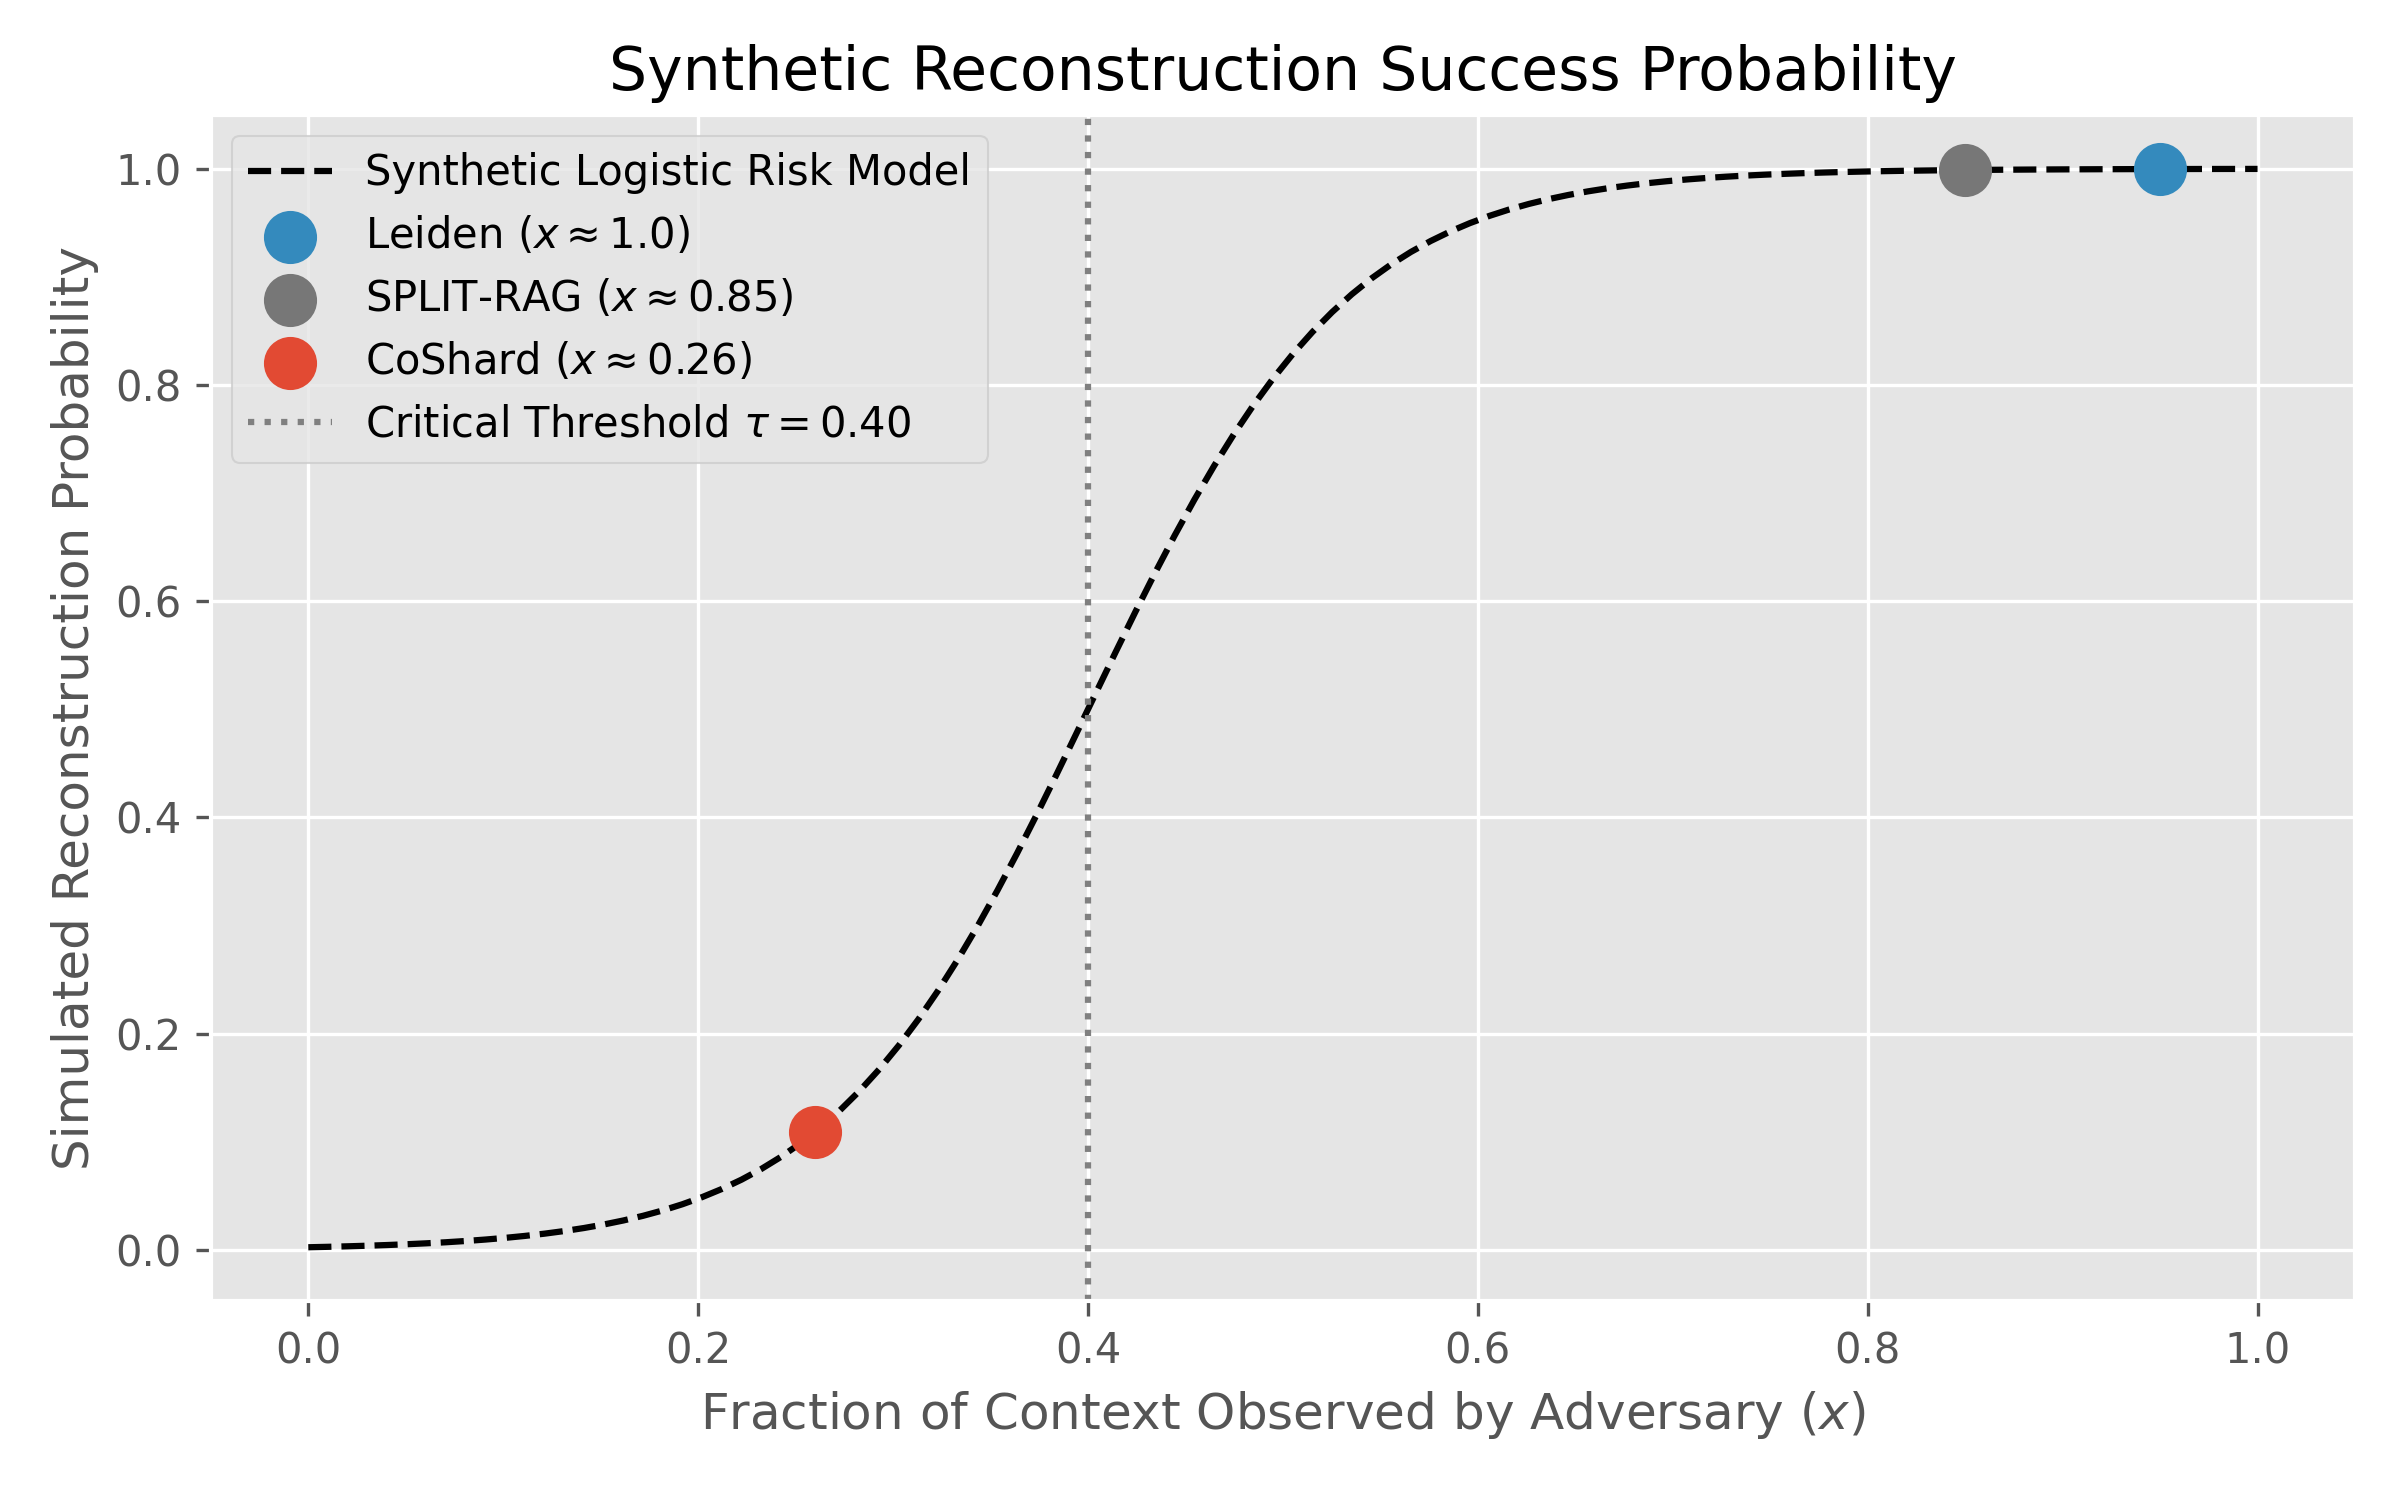
\includegraphics[width=\columnwidth]{figures/fig3_adversarial_success.png}}
\caption{Synthetic Reconstruction Success Probability. High-utility frameworks (K-Means, Leiden) yield high context concentration, resulting in near 100\% vulnerability in the simulation. CoShard successfully scatters the context, dropping the simulated success probability to $\sim$6\%.}
\label{fig:adversarial_success}
\end{figure}

As shown in Figure \ref{fig:adversarial_success}, standard Leiden and K-Means clustering hand the adversary nearly the entire topic, driving $x \to 1.0$ and yielding a near 100\% simulated success rate. CoShard leverages its SHADE-penalized objective function to distribute the topic graph smoothly across the network. Under CoShard, the maximum context observed by any single compromised shard is empirically bounded to $\rho \approx 0.26$. Because $0.26 \ll \tau$, the theoretical simulated success probability drops to a mere 6\%. Future work will validate these synthetic bounds using explicit end-to-end generative attacks, evaluating reconstructed text via ROUGE and BLEU metrics.
